{\Large {Preliminary Analysis}}
\\[0.125in]
The survey results from the publicly available data set are available in csv format on the EIA website, labeled as a microdata file. \footnote{\href{https://www.eia.gov/consumption/commercial/data/2012/index.php?view=microdata}{microdata - \url{https://www.eia.gov/consumption/commercial/data/2012/index.php?view=microdata}}}  This file consists of 6,720 records that represent an estimated 5.6 million total buildings in the United States, using a complex sampling design that is explained in detail in the user's guide.  This data set consists of 1,119 variables, which includes various major fuel consumption values, such as electricity, natural gas, etc.  From initial inspection on these proposed response variables, after normalizing per square foot, it appears that they have a unimodal right skew, and can possibly be modeled.\\

\begin{figure}[h]
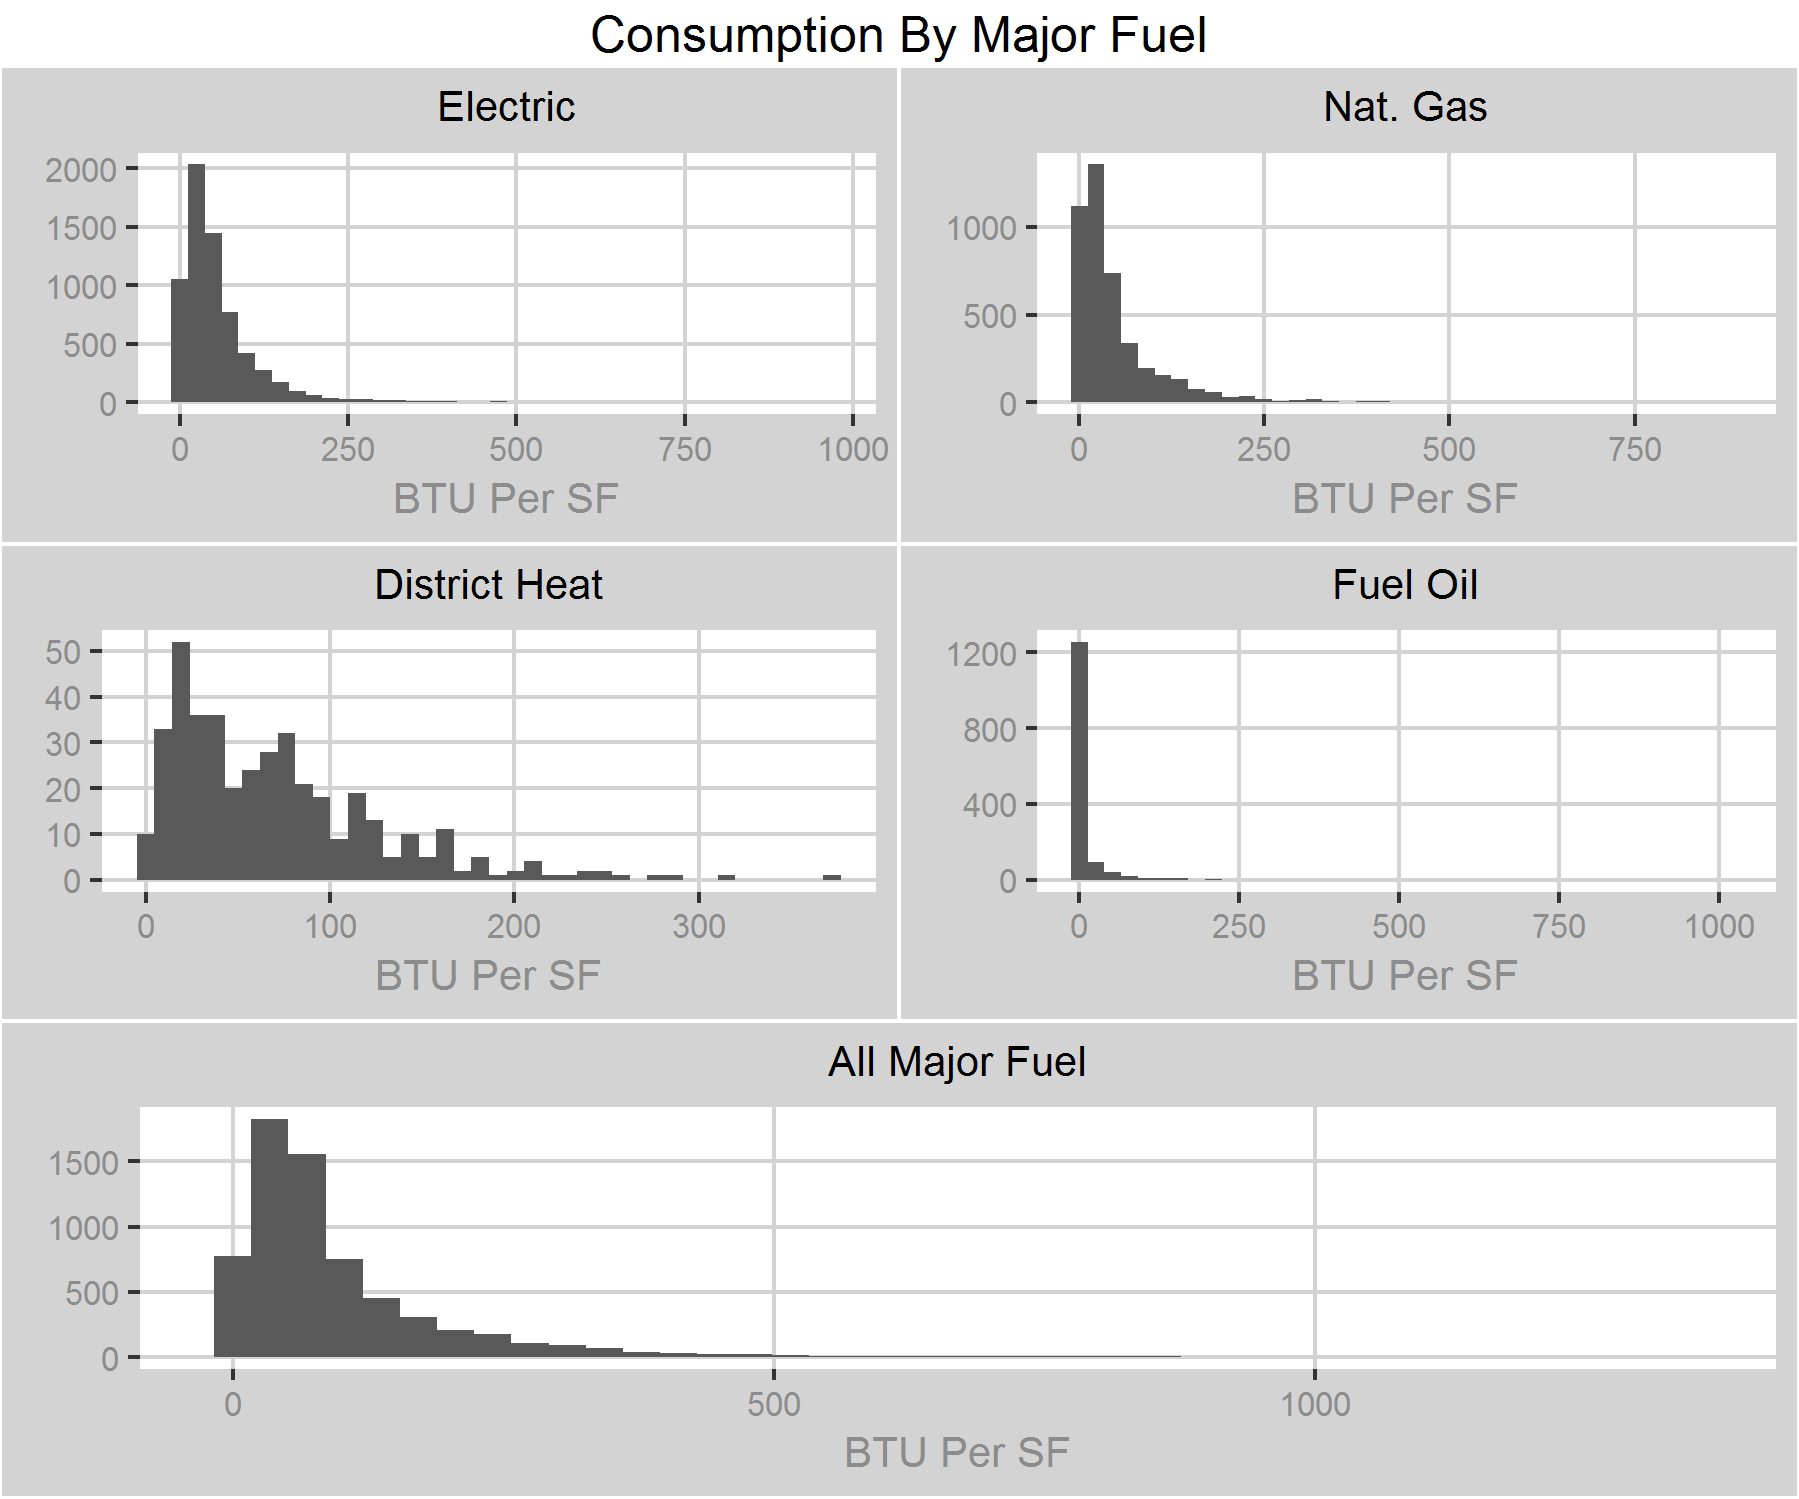
\includegraphics[width=\textwidth]{major_fuels_preliminary_analysis.png}
\centering
\end{figure}
